\documentclass[12pt,titlepage]{article}
%\usepackage[spanish]{babel}
%\usepackage[utf8]{inputenc}
%\usepackage[utf8]{inputenc}
\usepackage{amsmath}
\usepackage{amssymb}
\usepackage{graphicx}
%\usepackage{caratula}
\usepackage{float}
\usepackage{subfigure}
\usepackage{wrapfig}
\usepackage{listings}
%\usepackage{float}
\usepackage{xunicode,xltxtra,url,parskip}
\usepackage{fontspec}
\defaultfontfeatures{Mapping=tex-text}
\setmainfont[SmallCapsFont = Fontin SmallCaps]{Fontin}
\lstset{language=C,basicstyle=\small\tt,keywordstyle=\bf,tabsize=3,breaklines=true,linewidth=16cm,postbreak={\mbox{$\rightsquigarrow$}},prebreak={\mbox{$\rightsquigarrow$}}}

%\usepackage{a4wide}
%\usepackage{amssymb}
%\usepackage{amsmath}
 \usepackage{enumerate}
 \parindent = 12 pt
 \parskip = 12 pt
%\usepackage[width=15.5cm, left=3cm, top=2.5cm, height= 24.5cm]{geometry}

\usepackage{color}
\usepackage{url}
\definecolor{lnk}{rgb}{0,0,0.4}
\usepackage[colorlinks=true,linkcolor=lnk,citecolor=blue,urlcolor=blue]{hyperref}

\newcommand{\func}[2]{\texttt{#1}(#2) :}
\newcommand{\tab}{\hspace*{2em}}
\newcommand{\FOR}{\textbf{for }}
\newcommand{\TO}{\textbf{ to }}
\newcommand{\IF}{\textbf{if }}
\newcommand{\WHILE}{\textbf{while }}
\newcommand{\THEN}{\textbf{then }}
\newcommand{\ELSE}{\textbf{else }}
\newcommand{\RET}{\textbf{return }}
\newcommand{\MOD}{\textbf{ \% }}
\newcommand{\OR}{\textbf{ or }}
\newcommand{\NOT}{\textbf{ not }}
\newcommand{\tOde}[1]{\tab \small{\mathcal{O}($#1$)}}
\newcommand{\Ode}[1]{\ensuremath{\small{\mathcal{O}\left(#1\right)}}}
\newcommand{\VSP}{\vspace*{3em}}
\newcommand{\Pa}{\vspace{5mm}}
\newenvironment{pseudo}{\noindent\begin{tabular}{ll}}{\end{tabular}\VSP}

\newenvironment{while}{\WHILE \\ \setlength{\leftmargin}{0em} }{}

\newcommand{\iif}{\Leftrightarrow}
\newcommand{\gra}[1]{\noindent\includegraphics[scale=.70]{#1}\\}
\newcommand{\gras}[2]{\noindent\includegraphics[scale=#2]{#1}\\}
\newcommand{\grasize}[2]{\noindent\includegraphics[width=#2]{#1}\\}
\newcommand{\gram}[1]{\noindent\includegraphics[scale=.50]{#1}}
\newcommand{\dirmail}[1]{\normalsize{\texttt{#1}}}
\newenvironment{usection}[1]{\newpage\begin{section}*{#1}	\addcontentsline{toc}{section}{#1}}{\end{section}}
\newenvironment{ucsection}[1]{\newpage\begin{section}*{#1}	\addcontentsline{toc}{section}{#1}}{\end{section}}
\newenvironment{usubsection}[1]{\begin{subsection}*{#1}	\addcontentsline{toc}{subsection}{#1}}{\end{subsection}}

\newcommand{\superref}[1]{\textsuperscript{\ref{#1}}}

\addtolength{\topmargin}{-2cm}
\addtolength{\textheight}{3cm}

\begin{document}

\begin{titlepage}
\begin{center}
{\textbf{Universidad de Buenos Aires}\\Facultad de Ciencias Exactas y Naturales}

\vspace{1.5cm}

\begin{tabular}{r}
{\Large \bfseries Bases de Datos}\\
\hline
\textsc{\small 1er cuatrimestre 2011}\\
\end{tabular}
\vspace{2cm}

\begin{tabular}{l}
{\large TP1}\\
\textbf{\Huge DER, MR, SQL}\\
\end{tabular}

\vspace{1cm}

%\begin{minipage}[b]{0.7\linewidth}
%\begin{tabular}{l}
%\textbf{Abstract}\\
%{In this document we analyze the differences of the methods PSSM (Position-Specific Scoring Matrix) and ANN (Artificial neural networks) for Peptide MHC binding predictions.}\\
%\end{tabular}
%\end{minipage}

\vspace{1cm}

\begin{tabular}{lr}
Mariano Bianchi & \texttt{marianobianchi08@gmail.com}\\
Pablo Brusco & \texttt{pablo.brusco@gmail.com}\\
Julian Dondero & \texttt{juliandondero@gmail.com}\\
Kevin Allekotte & \texttt{kevinalle@gmail.com}\\
\end{tabular}

\vspace{2cm}

{\large Mayo 2011}

\end{center}
\end{titlepage}
\protect\setcounter{tocdepth}{1}
\tableofcontents
%\newpage

	\begin{ucsection}{DER}
		\begin{figure}[ht!]
			\noindent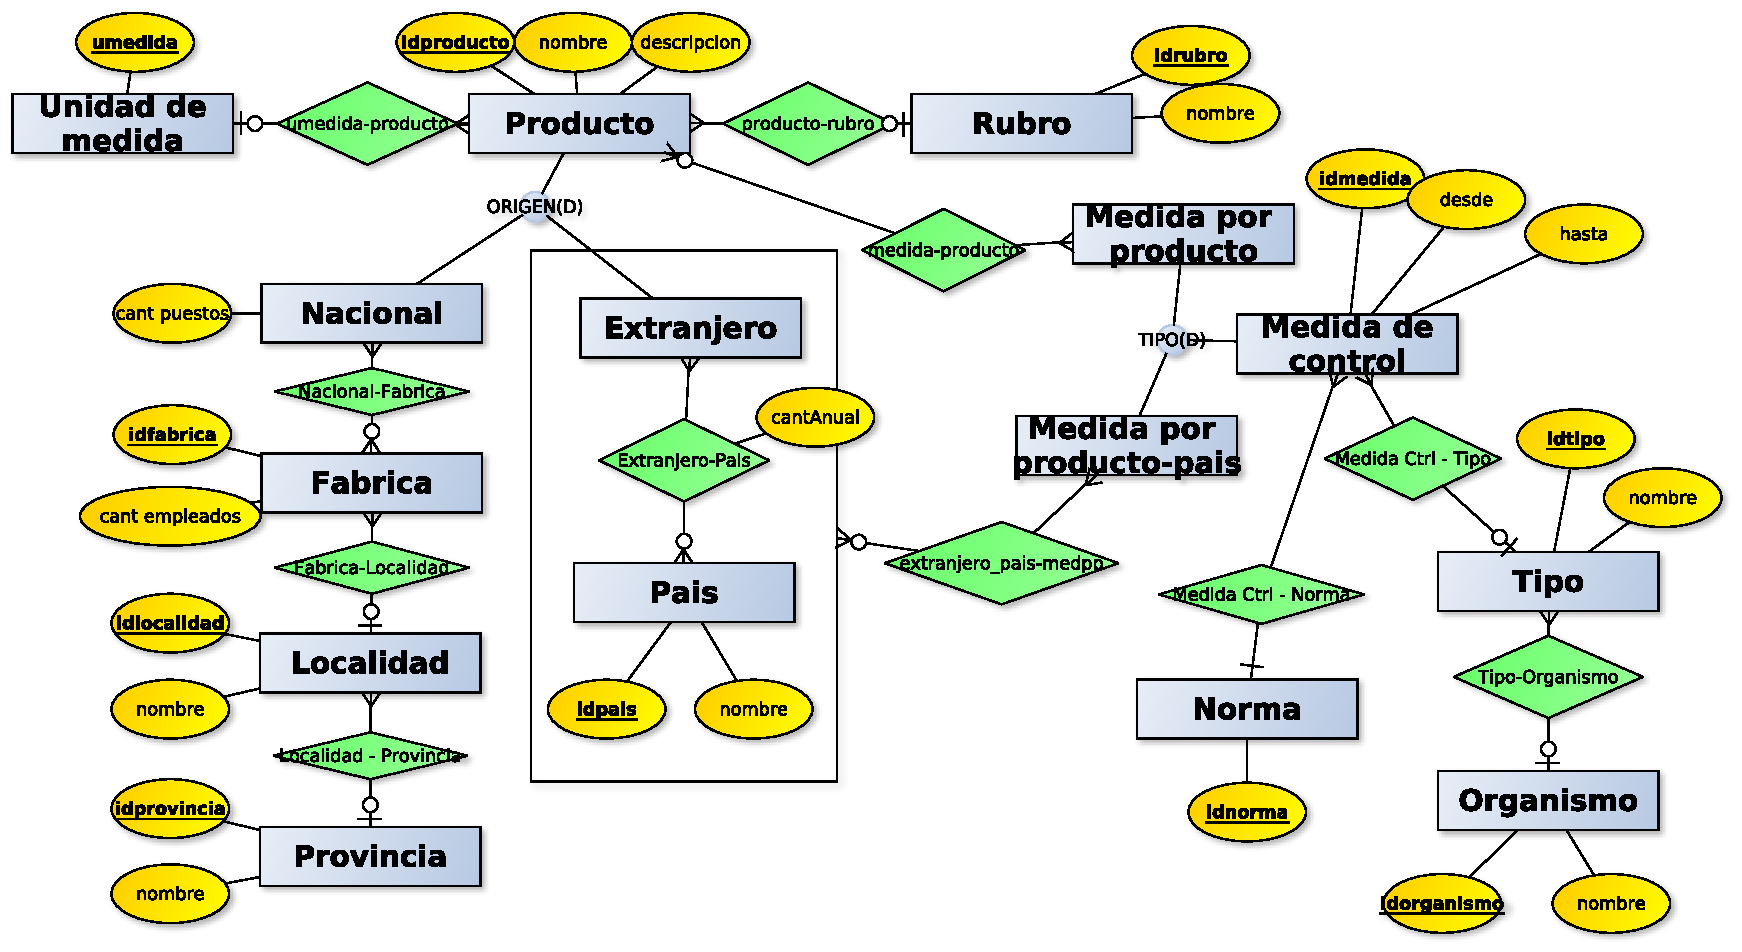
\includegraphics[angle=90,height=20cm]{der.pdf}
			\label{fig:der}
		\end{figure}
	\end{ucsection}
	
	\begin{ucsection}{MR}
		
	\end{ucsection}
	
	\begin{ucsection}{SQL}
		
	\end{ucsection}

\end{document}
